%AXIOMATIC MODEL DEMYSTIFIED----------------------------------------------

\documentclass[12pt, TexShade, letterpaper]{report}
\usepackage[utf8]{inputenc}
\usepackage{amsmath}
\usepackage{amssymb}
\usepackage{geometry}
\usepackage[dvipsnames]{xcolor}
\usepackage{graphicx}
\usepackage{tikz}
\usepackage{amsthm}
\usepackage{float}
\usepackage{centernot}
\usepackage{tasks}
\usepackage{fancyhdr}
\usepackage{lmodern}


% Overwrite the plain page style with a red line and page numbering
\fancypagestyle{plain}{%
	\fancyhf{} % clear all header and footer fields
	\fancyhead[R]{\textbf{\thepage}} % except the center
}

% Create the fancy page style header
\pagestyle{fancy}
\fancyhf{}
\lhead{\textbf{\nouppercase{\leftmark}}}
\chead{}
\rhead{\textbf{\thepage}}


% Set page numbering to roman
\setcounter{page}{2}\renewcommand{\thepage}{\roman{page}}

\author{\textcopyright Author, August, 2020}
\date{}


\usepackage{xpatch}
\xpretocmd\headrule{\color{red}}{}{\PatchFailed}





%Short form to use stack_relative
\newcommand{\stck}{\stackrel{\longrightarrow}}

%A different version of the above 
\newcommand{\stckdet}[1]{\stackrel{{#1}}}

%We write a lot of relations between two events using the orderings, so a short form to use that
\newcommand{\reln}[3]{#1\stck{_{#2}}#3}

%We use a more detailed version of the above relation to indicate direct / indirect relations 

\newcommand{\reldet}[4]{#1\stckdet{_{#2}}{{\stck{_{#3}}}}#4}

%We also will introduce a short form to write an event belongs to some set
\newcommand{\event}[2]{#1\!\in\!#2}

%To make events and their type more close to each other
\newcommand{\typ}[1]{\textit{#1}}
\newcommand{\et}[2]{#1\!:\!\typ{#2}}

%Short form to write color text
\newcommand{\critic}[2]{\textcolor{#1}{\footnotesize #2}}

%A new command to quickly use cons function in formal descriptions
\newcommand{\cons}[2]{\textit{cons}(#1,#2)}

%Useful command syntax
\newcommand{\rmw}{\textit{rmw}\,}
\newcommand{\set}[1]{\textbf{\textit{#1}}}

%Some preliminary latex commands to format writing theorems 
\newtheorem{lemma}{Lemma}

\newtheorem{theorem}{Theorem}[lemma]

\newtheorem{corollary}{Corollary}[theorem]

\newtheorem{definition}{Definition}

\newtheorem{property}{Property}


\begin{document}

\begin{titlepage}
    \begin{center}
        \vspace*{0.5cm}

        \LARGE
        \textbf{Analysis of the ECMAScript Memory Model : A Program Transformation Perspective}
        
        \vspace{1cm}
        
        \textit{Akshay Gopalakrishnan}
        
        \vspace{7cm}
        
        % \includegraphics[width=0.25\textwidth]{mcglogo.png}
        
        \Large
        School of Computer Science
        
        \vspace{5mm}
        McGill University
        
        \vspace{5mm}
    %	Montr\'eal, Qu\'ebec, Canada
        
        \vspace{5mm}
        August 15, 2020
        \small
        \vspace{0.5cm}
        {\color{red} \hrule height 0.75mm}
        
        \vspace{0.3cm}
        A thesis submitted to McGill University in partial fulfillment of the requirements of the degree of Computer Science
        
        \copyright\hspace{0.5mm}2020 Author
        
    \end{center}
\end{titlepage}

\setlength{\voffset}{2cm}
\renewcommand{\chaptermark}[1]{%
    \markboth{\thechapter.\ #1}{}}
    

    \chapter*{Abstract}\markboth{Abstract}{}
	\label{chap:engAbstract}
%	\addcontentsline{toc}{section}{\nameref{chap:engAbstract}}

\chapter*{Abrégé}\markboth{Abrégé}{}
	\label{chap:frAbstract}
%	\addcontentsline{toc}{section}{\nameref{chap:frAbstract}}

\chapter*{Acknowledgements}\markboth{Acknowledgements}{}
	\label{chap:acknowledgments}
%	\addcontentsline{toc}{section}{\nameref{chap:acknowledgments}}


 % Start of ToC, LoT, gls
 \tableofcontents\thispagestyle{plain}

 \listoffigures\thispagestyle{plain}
%	\addcontentsline{toc}{section}{\listfigurename}
 \listoftables
%	\addcontentsline{toc}{section}{\listtablename}

  \clearpage
 \pagenumbering{arabic} % restart page numbers at one, now in arabic style

    \chapter{Introduction}
    %
\section{Introduction}
    Instruction reordering is a common transformation done by the compiler/hardware, which is essential to optimizations such as instruction scheduling, loop invariant removal, partial redundancy elimination, etc. 
    However, whether we can do such reordering freely given a concurrent program using relaxed memory accesses is a bit unclear. 
     
    \paragraph{Simple reordering is not straightforward under shared memory semantics}
    The main reason is that memory accesses here, do not just perform the desired operation (i.e Read / Write) but also imply certain visibility guarantees across all the other threads.  
    In our observation, we find that, the relaxed memory model of ECMAScript prescribe semantics for visibility using the $\stck{_{hb}}$ relations. 
    
    \paragraph{Some Examples}
        We show a couple of examples to showcase why reordering may not be that straightforward. 
        Consider the first example in Figure~\ref{reord:example1(a)} below of a Candidate before and after reordering two events.
        The original candidate is to the left and that on the right is after reordering the two reads of $T2$.
        The observable behavior in question is written in the middle(orange box). 
        \begin{figure}[H]
            \centering
            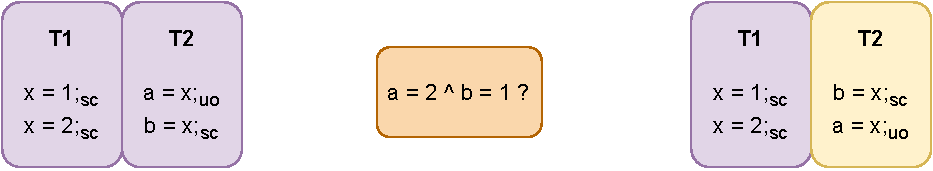
\includegraphics[scale=0.7]{5.InstructionReordering/0.Intro/ReorderingExample1(a).pdf}
            \caption{First example for reordering in candidates of the original program and its reordered counterpart.}
            \label{reord:example1(a)} 
        \end{figure}
        
        Figure~\ref{reord:example1(b)} has two sets of relations. 
        The first justifies the outcome for the reordered Candidate. 
        While the second justifies for the original Candidate. 
        Notice that in the first set of relations, we can infer that one may have a read memory ordered before a write that it reads from. 
        This is quite counter intuitive to understand at first. 
        But strictly from the semantics of the model, this justification to the observable behavior is completely valid\footnotemark. 
        \begin{figure}[H]
            \centering
            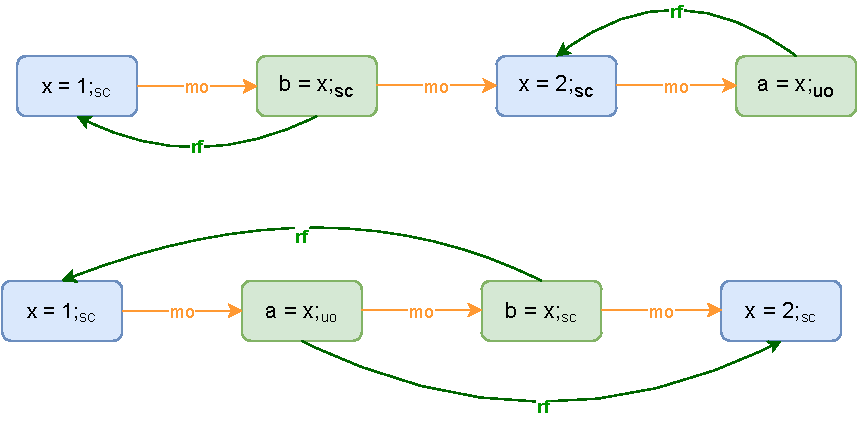
\includegraphics[scale=0.7]{5.InstructionReordering/0.Intro/ReorderingExample1(b).pdf}
            \caption{The set of partial order relations justifying the observable behavior in question for both the candidates in Figure~\ref{reord:example1(a)}.} 
            \label{reord:example1(b)}
        \end{figure}

        \footnotetext{In practice, this can be due to read speculation at the hardware level.}
        
        Consider another example in Figure~\ref{reord:example2(a)}.
        The figure on the left is the original candidate and that on the right is after reordering the two events of $T1$.
        The observable behavior in question is written in the middle(orange box). 
        \begin{figure}[H]
            \centering
            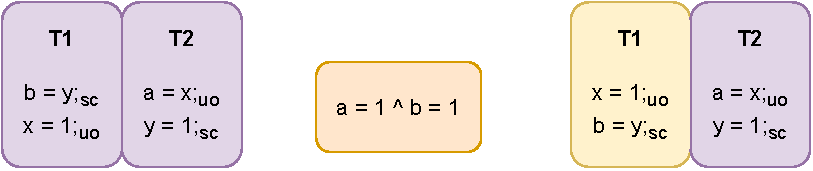
\includegraphics[scale=0.7]{5.InstructionReordering/0.Intro/ReorderingExample2(a).pdf}
            \caption{Second example for reordering with candidates of the original program and its reordered counterpart.} 
            \label{reord:example2(a)}
        \end{figure}
   
        Figure~\ref{reord:example2(b)} has two sets of relations. 
        The first justifies that such an outcome is not possible for the original program candidate due to Axiom \ref{CoRe}. 
        While the second justifies that this outcome is possible for the reordered program.
        Note that we cannot infer in the reordered candidate the set of relations for any candidate execution to have $\reln{a=x;_{uo}}{hb}{x=1;_{uo}}$. 
        \begin{figure}[H]
            \centering
            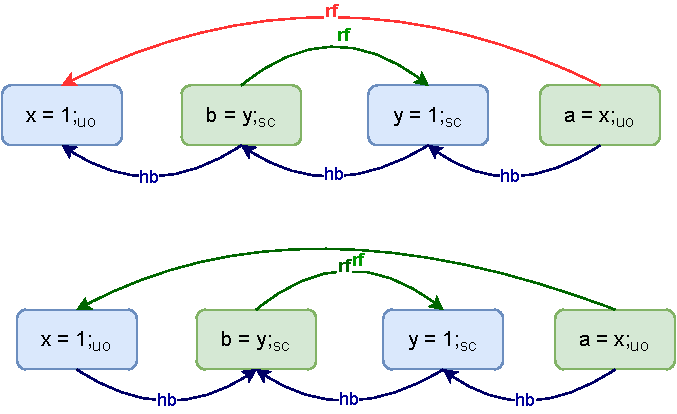
\includegraphics[scale=0.7]{5.InstructionReordering/0.Intro/ReorderingExample2(b).pdf}
            \caption{The set of partial order relations justifying the observable behavior in question for both the candidates in Figure~\ref{reord:example2(a)}.} 
            \label{reord:example2(b)}
        \end{figure}

        The above two examples show that we have to be careful while reordering two events in the same thread. 
        By example analysis, for each observable behavior, one must check all possible candidate executions and assert whether such an observable is possible or not. 
        This method of checking validity of reordering will scale exponentially as the program size increases. 
        It may also be the case that the compiler may not have information on which exact events would be executed in other threads to assert such reordering is valid. 

    
    
    
    
    

    \chapter{Background}

    \chapter{Related Work}

    \chapter{The Memory Model}
    %The ECMAScript Memory Model
    \section{Elimination}

    Many programs which contain loops or are representing big softwares fall victim to having many redundant code. 
    This could also be possible due to differnt phases of optimization the compiler performs, which leaves certain residual code in each phase.
    One such example of redundant code is that when there are two consecutive reads or writes writing the same value to the same memory location.
    Another example could be the case that after many optimization passes, certain memory values are not used by the program itself, so the compiler may decide to remove it.  
    In a sequential setting the effect of removing such code is nothing.
    However, as we saw for simple reordering too, in a concurrent setting, elimination may not be that straightforward. 
    
    Let us for instance consider a program where we have two consecutive writes to the same memory writing the same value and the program after eliminating the latter write as below. 

    %SHow example here 

    
    The orange box shows the possible outcome that we want to consider. 
    In the first program, such an outcome should not be allowed. 
    While in the program after eliminating the latter write, this outcome is allowed.
    The following figure explains the relations formed in a candidate execution that can justify the observable behavior in question. 
    
    %Show relations here relevant

    The first set of relations is for the original program, where Axiom \ref{CoRe} prohibits the read $a$ to have value of $y$ as $2$.
    The second set is for the modified program, where none of the axioms.
    
    %For reads
    %I still do not have a counter example to show that elimination of reads is not safe. 
    %This is because I do not yet understand the implications of this on observable behaviors. 
    %Typically, if we remove the read from the set of observables, nothing should change, that is, restrictions on events agent ordered before or after the read must remain as it is.
    %This is because removal of restrictions might lead to new observable behaviors. 
    %The only case where this is not okay is when the read is part of a loop conditional. 
    %Removing such reads from every candidate will resort to non-termination of code.
    %One can jot this down to just restricting elimination of reads that are part of conditionals.
    %But otherwise, one can still eliminate. 
    %I am not sure which other case can be taken. How about showing when two reads are memory ordered without happens-before? Then elimination will not have any use.
    %We can skip this part for now and just refine the previous chapter first.
    An example where reads is unsafe to be eliminated is not quite easy to construct.
    This is because the semantics of the model does not really have any read-read dependance; one read value does not affect any subsequent(agent ordered) read value to same memory unless constrained by happens-before.
    So one might assume that we can freely eliminate reads: this however would not be safe to do, due to other reasons such as forward progress.
    If for instance, a loop repeatedly checks the value of some memory (say $x$) and will terminate only if the memory reads some fixed value, each candidate execution representing each iteration of the loop would represent also the minimum iterations before the read is of fixed value. 
    And this value would be of the read in the last iteration. 
    

    There are two types of elimination we are concerned with:
    \begin{itemize}
        \item Read Elimination
        \item Write Elimination
    \end{itemize}

    We address each part separately.


    %Instruction reordering
    \chapter{Instruction Reordering}
    \input{InstructionReordering/reordering_opt.tex}

    %Elimination
    \chapter{Elimination} 
    
\section{Introduction}
    Instruction reordering is a common transformation done by the compiler/hardware, which is essential to optimizations such as instruction scheduling, loop invariant removal, partial redundancy elimination, etc. 
    However, whether we can do such reordering freely given a concurrent program using relaxed memory accesses is a bit unclear. 
     
    \paragraph{Simple reordering is not straightforward under shared memory semantics}
    The main reason is that memory accesses here, do not just perform the desired operation (i.e Read / Write) but also imply certain visibility guarantees across all the other threads.  
    In our observation, we find that, the relaxed memory model of ECMAScript prescribe semantics for visibility using the $\stck{_{hb}}$ relations. 
    
    \paragraph{Some Examples}
        We show a couple of examples to showcase why reordering may not be that straightforward. 
        Consider the first example in Figure~\ref{reord:example1(a)} below of a Candidate before and after reordering two events.
        The original candidate is to the left and that on the right is after reordering the two reads of $T2$.
        The observable behavior in question is written in the middle(orange box). 
        \begin{figure}[H]
            \centering
            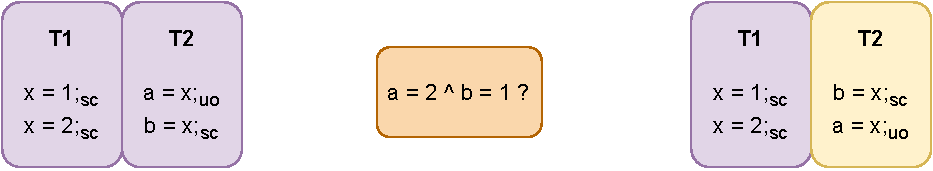
\includegraphics[scale=0.7]{5.InstructionReordering/0.Intro/ReorderingExample1(a).pdf}
            \caption{First example for reordering in candidates of the original program and its reordered counterpart.}
            \label{reord:example1(a)} 
        \end{figure}
        
        Figure~\ref{reord:example1(b)} has two sets of relations. 
        The first justifies the outcome for the reordered Candidate. 
        While the second justifies for the original Candidate. 
        Notice that in the first set of relations, we can infer that one may have a read memory ordered before a write that it reads from. 
        This is quite counter intuitive to understand at first. 
        But strictly from the semantics of the model, this justification to the observable behavior is completely valid\footnotemark. 
        \begin{figure}[H]
            \centering
            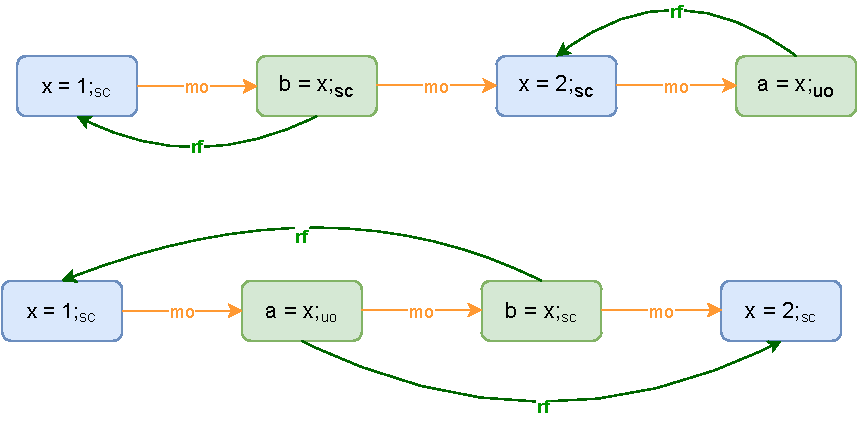
\includegraphics[scale=0.7]{5.InstructionReordering/0.Intro/ReorderingExample1(b).pdf}
            \caption{The set of partial order relations justifying the observable behavior in question for both the candidates in Figure~\ref{reord:example1(a)}.} 
            \label{reord:example1(b)}
        \end{figure}

        \footnotetext{In practice, this can be due to read speculation at the hardware level.}
        
        Consider another example in Figure~\ref{reord:example2(a)}.
        The figure on the left is the original candidate and that on the right is after reordering the two events of $T1$.
        The observable behavior in question is written in the middle(orange box). 
        \begin{figure}[H]
            \centering
            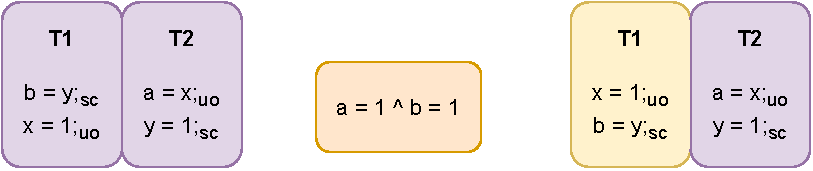
\includegraphics[scale=0.7]{5.InstructionReordering/0.Intro/ReorderingExample2(a).pdf}
            \caption{Second example for reordering with candidates of the original program and its reordered counterpart.} 
            \label{reord:example2(a)}
        \end{figure}
   
        Figure~\ref{reord:example2(b)} has two sets of relations. 
        The first justifies that such an outcome is not possible for the original program candidate due to Axiom \ref{CoRe}. 
        While the second justifies that this outcome is possible for the reordered program.
        Note that we cannot infer in the reordered candidate the set of relations for any candidate execution to have $\reln{a=x;_{uo}}{hb}{x=1;_{uo}}$. 
        \begin{figure}[H]
            \centering
            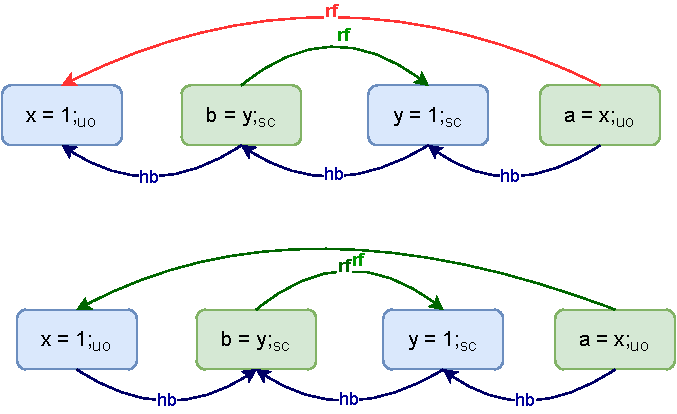
\includegraphics[scale=0.7]{5.InstructionReordering/0.Intro/ReorderingExample2(b).pdf}
            \caption{The set of partial order relations justifying the observable behavior in question for both the candidates in Figure~\ref{reord:example2(a)}.} 
            \label{reord:example2(b)}
        \end{figure}

        The above two examples show that we have to be careful while reordering two events in the same thread. 
        By example analysis, for each observable behavior, one must check all possible candidate executions and assert whether such an observable is possible or not. 
        This method of checking validity of reordering will scale exponentially as the program size increases. 
        It may also be the case that the compiler may not have information on which exact events would be executed in other threads to assert such reordering is valid. 

    
    
    
    
    

    \chapter{Our Critique of The Model}

    \chapter{Conclusion, Summary, Future Work}

\end{document}
